\documentclass[1p]{elsarticle_modified}
%\bibliographystyle{elsarticle-num}

%\usepackage[colorlinks]{hyperref}
%\usepackage{abbrmath_seonhwa} %\Abb, \Ascr, \Acal ,\Abf, \Afrak
\usepackage{amsfonts}
\usepackage{amssymb}
\usepackage{amsmath}
\usepackage{amsthm}
\usepackage{scalefnt}
\usepackage{amsbsy}
\usepackage{kotex}
\usepackage{caption}
\usepackage{subfig}
\usepackage{color}
\usepackage{graphicx}
\usepackage{xcolor} %% white, black, red, green, blue, cyan, magenta, yellow
\usepackage{float}
\usepackage{setspace}
\usepackage{hyperref}

\usepackage{tikz}
\usetikzlibrary{arrows}

\usepackage{multirow}
\usepackage{array} % fixed length table
\usepackage{hhline}

%%%%%%%%%%%%%%%%%%%%%
\makeatletter
\renewcommand*\env@matrix[1][\arraystretch]{%
	\edef\arraystretch{#1}%
	\hskip -\arraycolsep
	\let\@ifnextchar\new@ifnextchar
	\array{*\c@MaxMatrixCols c}}
\makeatother %https://tex.stackexchange.com/questions/14071/how-can-i-increase-the-line-spacing-in-a-matrix
%%%%%%%%%%%%%%%

\usepackage[normalem]{ulem}

\newcommand{\msout}[1]{\ifmmode\text{\sout{\ensuremath{#1}}}\else\sout{#1}\fi}
%SOURCE: \msout is \stkout macro in https://tex.stackexchange.com/questions/20609/strikeout-in-math-mode

\newcommand{\cancel}[1]{
	\ifmmode
	{\color{red}\msout{#1}}
	\else
	{\color{red}\sout{#1}}
	\fi
}

\newcommand{\add}[1]{
	{\color{blue}\uwave{#1}}
}

\newcommand{\replace}[2]{
	\ifmmode
	{\color{red}\msout{#1}}{\color{blue}\uwave{#2}}
	\else
	{\color{red}\sout{#1}}{\color{blue}\uwave{#2}}
	\fi
}

\newcommand{\Sol}{\mathcal{S}} %segment
\newcommand{\D}{D} %diagram
\newcommand{\A}{\mathcal{A}} %arc


%%%%%%%%%%%%%%%%%%%%%%%%%%%%%5 test

\def\sl{\operatorname{\textup{SL}}(2,\Cbb)}
\def\psl{\operatorname{\textup{PSL}}(2,\Cbb)}
\def\quan{\mkern 1mu \triangleright \mkern 1mu}

\theoremstyle{definition}
\newtheorem{thm}{Theorem}[section]
\newtheorem{prop}[thm]{Proposition}
\newtheorem{lem}[thm]{Lemma}
\newtheorem{ques}[thm]{Question}
\newtheorem{cor}[thm]{Corollary}
\newtheorem{defn}[thm]{Definition}
\newtheorem{exam}[thm]{Example}
\newtheorem{rmk}[thm]{Remark}
\newtheorem{alg}[thm]{Algorithm}

\newcommand{\I}{\sqrt{-1}}
\begin{document}

%\begin{frontmatter}
%
%\title{Boundary parabolic representations of knots up to 8 crossings}
%
%%% Group authors per affiliation:
%\author{Yunhi Cho} 
%\address{Department of Mathematics, University of Seoul, Seoul, Korea}
%\ead{yhcho@uos.ac.kr}
%
%
%\author{Seonhwa Kim} %\fnref{s_kim}}
%\address{Center for Geometry and Physics, Institute for Basic Science, Pohang, 37673, Korea}
%\ead{ryeona17@ibs.re.kr}
%
%\author{Hyuk Kim}
%\address{Department of Mathematical Sciences, Seoul National University, Seoul 08826, Korea}
%\ead{hyukkim@snu.ac.kr}
%
%\author{Seokbeom Yoon}
%\address{Department of Mathematical Sciences, Seoul National University, Seoul, 08826,  Korea}
%\ead{sbyoon15@snu.ac.kr}
%
%\begin{abstract}
%We find all boundary parabolic representation of knots up to 8 crossings.
%
%\end{abstract}
%\begin{keyword}
%    \MSC[2010] 57M25 
%\end{keyword}
%
%\end{frontmatter}

%\linenumbers
%\tableofcontents
%
\newcommand\colored[1]{\textcolor{white}{\rule[-0.35ex]{0.8em}{1.4ex}}\kern-0.8em\color{red} #1}%
%\newcommand\colored[1]{\textcolor{white}{ #1}\kern-2.17ex	\textcolor{white}{ #1}\kern-1.81ex	\textcolor{white}{ #1}\kern-2.15ex\color{red}#1	}

{\Large $\underline{11n_{97}~(K11n_{97})}$}

\setlength{\tabcolsep}{10pt}
\renewcommand{\arraystretch}{1.6}
\vspace{1cm}\begin{tabular}{m{100pt}>{\centering\arraybackslash}m{274pt}}
\multirow{5}{120pt}{
	\centering
	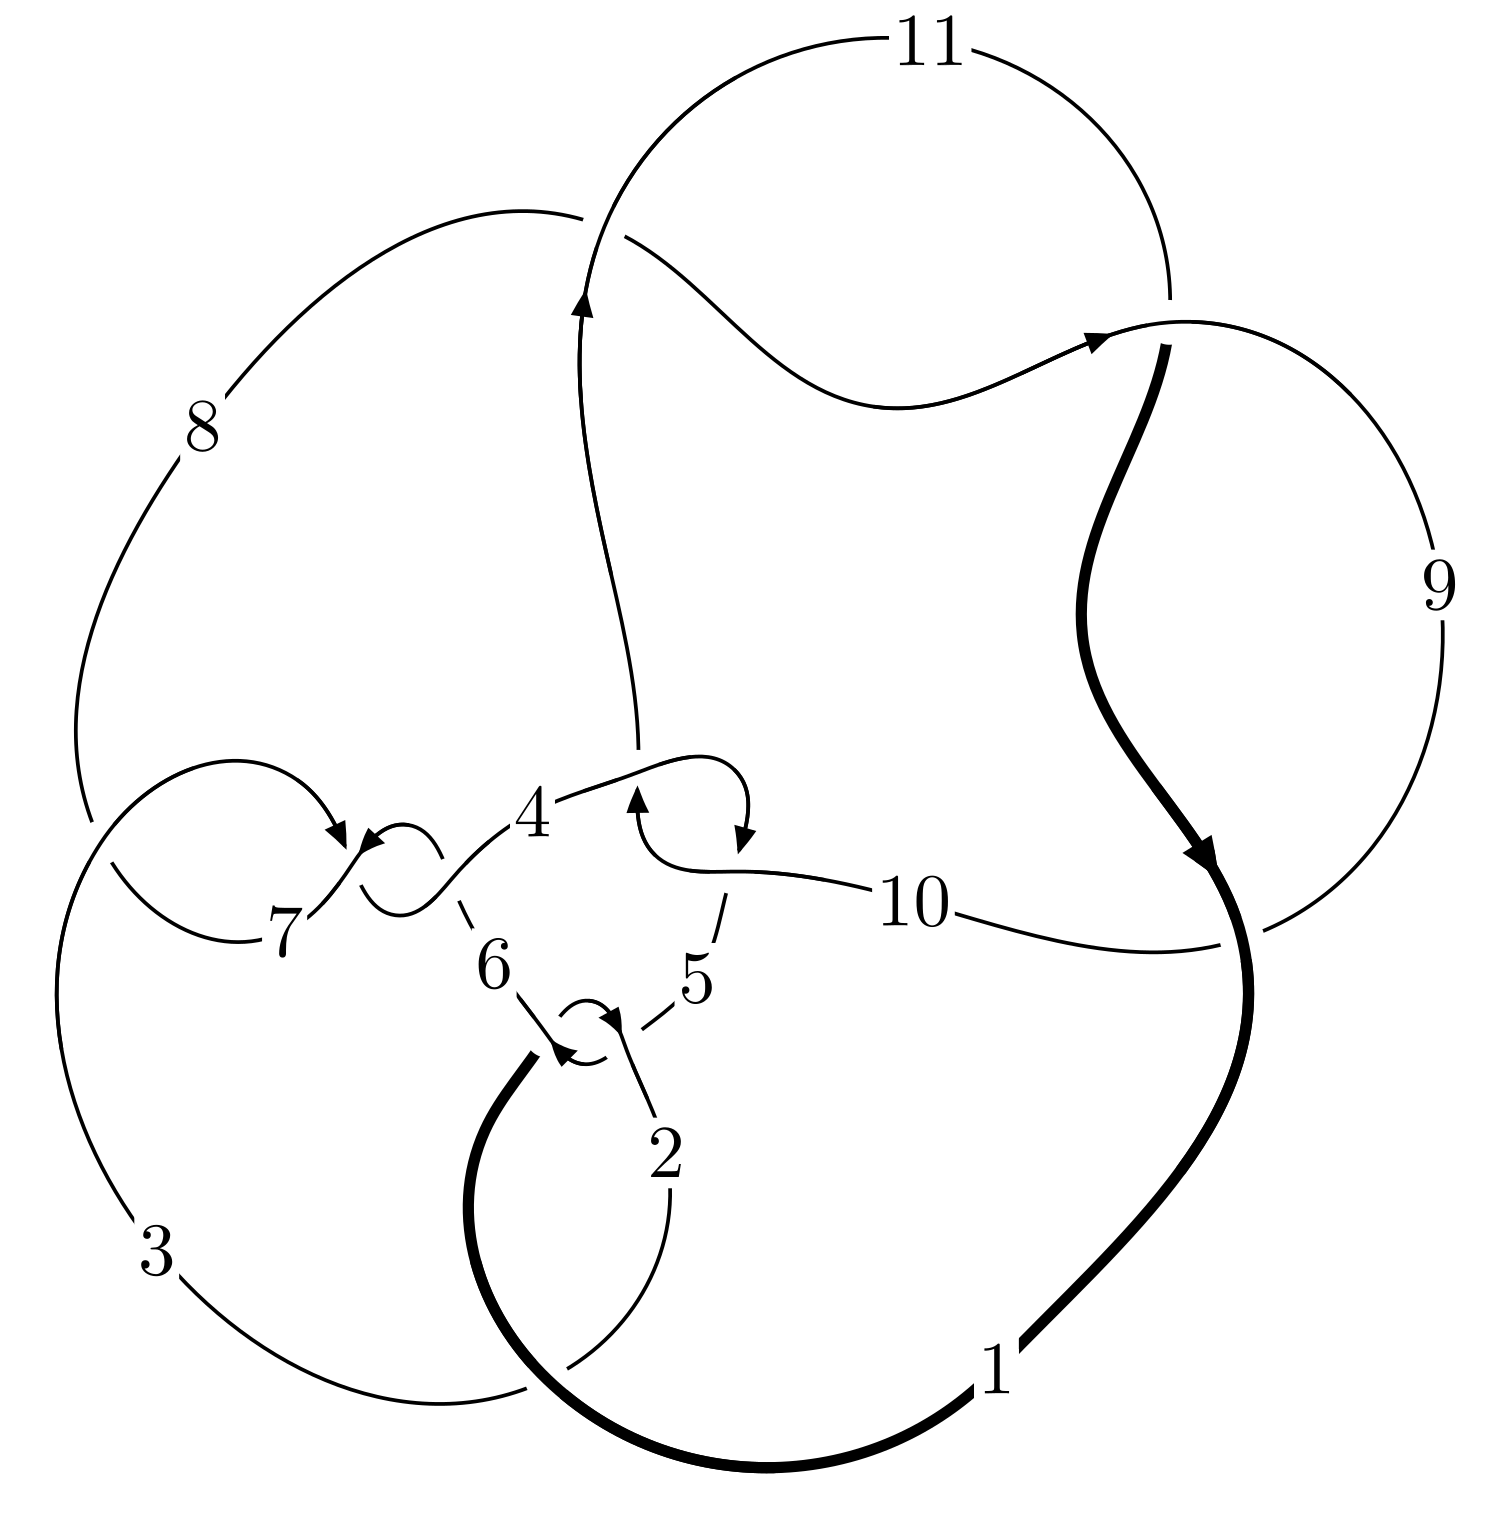
\includegraphics[width=112pt]{../../../GIT/diagram.site/Diagrams/png/713_11n_97.png}\\
\ \ \ A knot diagram\footnotemark}&
\allowdisplaybreaks
\textbf{Linearized knot diagam} \\
\cline{2-2}
 &
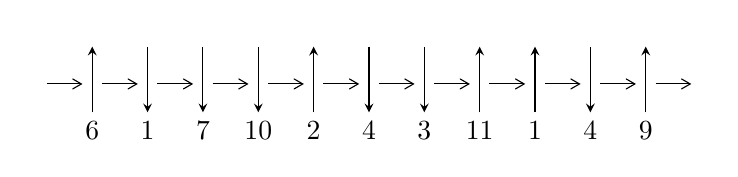
\begin{tikzpicture}[x=20pt, y=17pt]
	% nodes
	\node (C0) at (0, 0) {};
	\node (C1) at (1, 0) {};
	\node (C1U) at (1, +1) {};
	\node (C1D) at (1, -1) {6};

	\node (C2) at (2, 0) {};
	\node (C2U) at (2, +1) {};
	\node (C2D) at (2, -1) {1};

	\node (C3) at (3, 0) {};
	\node (C3U) at (3, +1) {};
	\node (C3D) at (3, -1) {7};

	\node (C4) at (4, 0) {};
	\node (C4U) at (4, +1) {};
	\node (C4D) at (4, -1) {10};

	\node (C5) at (5, 0) {};
	\node (C5U) at (5, +1) {};
	\node (C5D) at (5, -1) {2};

	\node (C6) at (6, 0) {};
	\node (C6U) at (6, +1) {};
	\node (C6D) at (6, -1) {4};

	\node (C7) at (7, 0) {};
	\node (C7U) at (7, +1) {};
	\node (C7D) at (7, -1) {3};

	\node (C8) at (8, 0) {};
	\node (C8U) at (8, +1) {};
	\node (C8D) at (8, -1) {11};

	\node (C9) at (9, 0) {};
	\node (C9U) at (9, +1) {};
	\node (C9D) at (9, -1) {1};

	\node (C10) at (10, 0) {};
	\node (C10U) at (10, +1) {};
	\node (C10D) at (10, -1) {4};

	\node (C11) at (11, 0) {};
	\node (C11U) at (11, +1) {};
	\node (C11D) at (11, -1) {9};
	\node (C12) at (12, 0) {};

	% arrows
	\draw[->,>={angle 60}]
	(C0) edge (C1) (C1) edge (C2) (C2) edge (C3) (C3) edge (C4) (C4) edge (C5) (C5) edge (C6) (C6) edge (C7) (C7) edge (C8) (C8) edge (C9) (C9) edge (C10) (C10) edge (C11) (C11) edge (C12) ;	\draw[->,>=stealth]
	(C1D) edge (C1U) (C2U) edge (C2D) (C3U) edge (C3D) (C4U) edge (C4D) (C5D) edge (C5U) (C6U) edge (C6D) (C7U) edge (C7D) (C8D) edge (C8U) (C9D) edge (C9U) (C10U) edge (C10D) (C11D) edge (C11U) ;
	\end{tikzpicture} \\
\hhline{~~} \\& 
\textbf{Solving Sequence} \\ \cline{2-2} 
 &
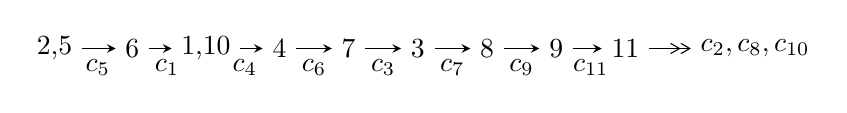
\begin{tikzpicture}[x=25pt, y=7pt]
	% node
	\node (A0) at (-1/8, 0) {2,5};
	\node (A1) at (1, 0) {6};
	\node (A2) at (33/16, 0) {1,10};
	\node (A3) at (25/8, 0) {4};
	\node (A4) at (33/8, 0) {7};
	\node (A5) at (41/8, 0) {3};
	\node (A6) at (49/8, 0) {8};
	\node (A7) at (57/8, 0) {9};
	\node (A8) at (65/8, 0) {11};
	\node (C1) at (1/2, -1) {$c_{5}$};
	\node (C2) at (3/2, -1) {$c_{1}$};
	\node (C3) at (21/8, -1) {$c_{4}$};
	\node (C4) at (29/8, -1) {$c_{6}$};
	\node (C5) at (37/8, -1) {$c_{3}$};
	\node (C6) at (45/8, -1) {$c_{7}$};
	\node (C7) at (53/8, -1) {$c_{9}$};
	\node (C8) at (61/8, -1) {$c_{11}$};
	\node (A9) at (10, 0) {$c_{2},c_{8},c_{10}$};

	% edge
	\draw[->,>=stealth]	
	(A0) edge (A1) (A1) edge (A2) (A2) edge (A3) (A3) edge (A4) (A4) edge (A5) (A5) edge (A6) (A6) edge (A7) (A7) edge (A8) ;
	\draw[->>,>={angle 60}]	
	(A8) edge (A9);
\end{tikzpicture} \\ 

\end{tabular} \\

\footnotetext{
The image of knot diagram is generated by the software ``\textbf{Draw programme}" developed by Andrew Bartholomew(\url{http://www.layer8.co.uk/maths/draw/index.htm\#Running-draw}), where we modified some parts for our purpose(\url{https://github.com/CATsTAILs/LinksPainter}).
}\phantom \\ \newline 
\centering \textbf{Ideals for irreducible components\footnotemark of $X_{\text{par}}$} 
 
\begin{align*}
I^u_{1}&=\langle 
-30727 u^{11}-34887 u^{10}+\cdots+3039144 b-2595171,\\
\phantom{I^u_{1}}&\phantom{= \langle  }-4836461 u^{11}+12982939 u^{10}+\cdots+36469728 a+72471903,\\
\phantom{I^u_{1}}&\phantom{= \langle  }u^{12}-2 u^{11}+11 u^{10}-18 u^9+46 u^8-52 u^7+89 u^6-74 u^5+120 u^4-38 u^3+52 u^2+9\rangle \\
I^u_{2}&=\langle 
b,\;- u^3-2 u^2+2 a-3 u-1,\;u^4+u^3+u^2+1\rangle \\
I^u_{3}&=\langle 
- a u+b+u+1,\;a^2+2 a u- a- u-2,\;u^2+1\rangle \\
\\
\end{align*}
\raggedright * 3 irreducible components of $\dim_{\mathbb{C}}=0$, with total 20 representations.\\
\footnotetext{All coefficients of polynomials are rational numbers. But the coefficients are sometimes approximated in decimal forms when there is not enough margin.}
\newpage
\renewcommand{\arraystretch}{1}
\centering \section*{I. $I^u_{1}= \langle -3.07\times10^{4} u^{11}-3.49\times10^{4} u^{10}+\cdots+3.04\times10^{6} b-2.60\times10^{6},\;-4.84\times10^{6} u^{11}+1.30\times10^{7} u^{10}+\cdots+3.65\times10^{7} a+7.25\times10^{7},\;u^{12}-2 u^{11}+\cdots+52 u^2+9 \rangle$}
\flushleft \textbf{(i) Arc colorings}\\
\begin{tabular}{m{7pt} m{180pt} m{7pt} m{180pt} }
\flushright $a_{2}=$&$\begin{pmatrix}0\\u\end{pmatrix}$ \\
\flushright $a_{5}=$&$\begin{pmatrix}1\\0\end{pmatrix}$ \\
\flushright $a_{6}=$&$\begin{pmatrix}1\\- u^2\end{pmatrix}$ \\
\flushright $a_{1}=$&$\begin{pmatrix}- u\\u^3+u\end{pmatrix}$ \\
\flushright $a_{10}=$&$\begin{pmatrix}0.132616 u^{11}-0.355992 u^{10}+\cdots+7.05457 u-1.98718\\0.0101104 u^{11}+0.0114792 u^{10}+\cdots-0.601162 u+0.853915\end{pmatrix}$ \\
\flushright $a_{4}=$&$\begin{pmatrix}-0.103120 u^{11}+0.218828 u^{10}+\cdots-3.36335 u+0.0167258\\0.0178412 u^{11}-0.0449113 u^{10}+\cdots+1.11635 u+0.000284291\end{pmatrix}$ \\
\flushright $a_{7}=$&$\begin{pmatrix}-0.0000315878 u^{11}+0.0179044 u^{10}+\cdots-0.854914 u+2.11635\\0.00740208 u^{11}-0.0289272 u^{10}+\cdots+0.112721 u-0.541350\end{pmatrix}$ \\
\flushright $a_{3}=$&$\begin{pmatrix}- u^3\\u^5+u^3+u\end{pmatrix}$ \\
\flushright $a_{8}=$&$\begin{pmatrix}0.0217851 u^{11}-0.0147232 u^{10}+\cdots-0.838473 u+2.20500\\0.0577531 u^{11}-0.0685147 u^{10}+\cdots+0.179624 u-0.829029\end{pmatrix}$ \\
\flushright $a_{9}=$&$\begin{pmatrix}0.149942 u^{11}-0.378276 u^{10}+\cdots+8.21373 u-2.31454\\-0.0310324 u^{11}+0.110398 u^{10}+\cdots-1.60439 u+1.29258\end{pmatrix}$ \\
\flushright $a_{11}=$&$\begin{pmatrix}0.167308 u^{11}-0.446132 u^{10}+\cdots+7.46196 u-1.32551\\-0.00135137 u^{11}-0.00746559 u^{10}+\cdots-1.11597 u+0.589375\end{pmatrix}$\\ \flushright $a_{11}=$&$\begin{pmatrix}0.167308 u^{11}-0.446132 u^{10}+\cdots+7.46196 u-1.32551\\-0.00135137 u^{11}-0.00746559 u^{10}+\cdots-1.11597 u+0.589375\end{pmatrix}$\\&\end{tabular}
\flushleft \textbf{(ii) Obstruction class $= -1$}\\~\\
\flushleft \textbf{(iii) Cusp Shapes $= \frac{4442973}{8104384} u^{11}-\frac{9147283}{8104384} u^{10}+\cdots+\frac{28543939}{8104384} u+\frac{25892857}{8104384}$}\\~\\
\newpage\renewcommand{\arraystretch}{1}
\flushleft \textbf{(iv) u-Polynomials at the component}\newline \\
\begin{tabular}{m{50pt}|m{274pt}}
Crossings & \hspace{64pt}u-Polynomials at each crossing \\
\hline $$\begin{aligned}c_{1},c_{5}\end{aligned}$$&$\begin{aligned}
&u^{12}-2 u^{11}+\cdots+52 u^2+9
\end{aligned}$\\
\hline $$\begin{aligned}c_{2}\end{aligned}$$&$\begin{aligned}
&u^{12}+18 u^{11}+\cdots+936 u+81
\end{aligned}$\\
\hline $$\begin{aligned}c_{3},c_{6},c_{7}\end{aligned}$$&$\begin{aligned}
&u^{12}-2 u^{11}+\cdots+12 u+9
\end{aligned}$\\
\hline $$\begin{aligned}c_{4},c_{10}\end{aligned}$$&$\begin{aligned}
&u^{12}-8 u^{11}+\cdots-48 u+64
\end{aligned}$\\
\hline $$\begin{aligned}c_{8},c_{9},c_{11}\end{aligned}$$&$\begin{aligned}
&u^{12}+7 u^{11}+\cdots-3 u+4
\end{aligned}$\\
\hline
\end{tabular}\\~\\
\newpage\renewcommand{\arraystretch}{1}
\flushleft \textbf{(v) Riley Polynomials at the component}\newline \\
\begin{tabular}{m{50pt}|m{274pt}}
Crossings & \hspace{64pt}Riley Polynomials at each crossing \\
\hline $$\begin{aligned}c_{1},c_{5}\end{aligned}$$&$\begin{aligned}
&y^{12}+18 y^{11}+\cdots+936 y+81
\end{aligned}$\\
\hline $$\begin{aligned}c_{2}\end{aligned}$$&$\begin{aligned}
&y^{12}-42 y^{11}+\cdots-88128 y+6561
\end{aligned}$\\
\hline $$\begin{aligned}c_{3},c_{6},c_{7}\end{aligned}$$&$\begin{aligned}
&y^{12}+2 y^{11}+\cdots+648 y+81
\end{aligned}$\\
\hline $$\begin{aligned}c_{4},c_{10}\end{aligned}$$&$\begin{aligned}
&y^{12}-30 y^{11}+\cdots+13056 y+4096
\end{aligned}$\\
\hline $$\begin{aligned}c_{8},c_{9},c_{11}\end{aligned}$$&$\begin{aligned}
&y^{12}- y^{11}+\cdots+559 y+16
\end{aligned}$\\
\hline
\end{tabular}\\~\\
\newpage\flushleft \textbf{(vi) Complex Volumes and Cusp Shapes}
$$\begin{array}{c|c|c}  
\text{Solutions to }I^u_{1}& \I (\text{vol} + \sqrt{-1}CS) & \text{Cusp shape}\\
 \hline 
\begin{aligned}
u &= \phantom{-}0.217703 + 0.714491 I \\
a &= -0.323268 - 0.564378 I \\
b &= -0.299646 + 0.378751 I\end{aligned}
 & -0.382669 + 1.142140 I & -4.20479 - 6.27644 I \\ \hline\begin{aligned}
u &= \phantom{-}0.217703 - 0.714491 I \\
a &= -0.323268 + 0.564378 I \\
b &= -0.299646 - 0.378751 I\end{aligned}
 & -0.382669 - 1.142140 I & -4.20479 + 6.27644 I \\ \hline\begin{aligned}
u &= -0.640918 + 1.176710 I \\
a &= -0.126668 - 0.646625 I \\
b &= \phantom{-}0.682857 - 1.234360 I\end{aligned}
 & \phantom{-}9.18153 - 2.19341 I & \phantom{-}4.66853 + 1.23820 I \\ \hline\begin{aligned}
u &= -0.640918 - 1.176710 I \\
a &= -0.126668 + 0.646625 I \\
b &= \phantom{-}0.682857 + 1.234360 I\end{aligned}
 & \phantom{-}9.18153 + 2.19341 I & \phantom{-}4.66853 - 1.23820 I \\ \hline\begin{aligned}
u &= \phantom{-}1.15244 + 0.97674 I \\
a &= -0.320357 + 0.241963 I \\
b &= \phantom{-}1.73050 + 0.90375 I\end{aligned}
 & -1.62774 + 2.71130 I & \phantom{-}0.00178 - 2.31651 I \\ \hline\begin{aligned}
u &= \phantom{-}1.15244 - 0.97674 I \\
a &= -0.320357 - 0.241963 I \\
b &= \phantom{-}1.73050 - 0.90375 I\end{aligned}
 & -1.62774 - 2.71130 I & \phantom{-}0.00178 + 2.31651 I \\ \hline\begin{aligned}
u &= -0.148425 + 0.443858 I \\
a &= \phantom{-}0.38903 + 3.01143 I \\
b &= \phantom{-}0.403960 - 0.536532 I\end{aligned}
 & \phantom{-}2.12411 - 0.85388 I & \phantom{-}7.33787 - 1.04083 I \\ \hline\begin{aligned}
u &= -0.148425 - 0.443858 I \\
a &= \phantom{-}0.38903 - 3.01143 I \\
b &= \phantom{-}0.403960 + 0.536532 I\end{aligned}
 & \phantom{-}2.12411 + 0.85388 I & \phantom{-}7.33787 + 1.04083 I \\ \hline\begin{aligned}
u &= \phantom{-}0.62854 + 1.75953 I \\
a &= -1.237110 - 0.324756 I \\
b &= -2.03160 + 1.52165 I\end{aligned}
 & -9.75530 + 10.18300 I & \phantom{-}1.33053 - 4.09142 I \\ \hline\begin{aligned}
u &= \phantom{-}0.62854 - 1.75953 I \\
a &= -1.237110 + 0.324756 I \\
b &= -2.03160 - 1.52165 I\end{aligned}
 & -9.75530 - 10.18300 I & \phantom{-}1.33053 + 4.09142 I\\
 \hline 
 \end{array}$$\newpage$$\begin{array}{c|c|c}  
\text{Solutions to }I^u_{1}& \I (\text{vol} + \sqrt{-1}CS) & \text{Cusp shape}\\
 \hline 
\begin{aligned}
u &= -0.20933 + 2.25945 I \\
a &= \phantom{-}1.035040 - 0.220318 I \\
b &= \phantom{-}3.51393 - 0.31919 I\end{aligned}
 & -12.69940 - 0.47600 I & -0.258917 + 0.098219 I \\ \hline\begin{aligned}
u &= -0.20933 - 2.25945 I \\
a &= \phantom{-}1.035040 + 0.220318 I \\
b &= \phantom{-}3.51393 + 0.31919 I\end{aligned}
 & -12.69940 + 0.47600 I & -0.258917 - 0.098219 I\\
 \hline 
 \end{array}$$\newpage\newpage\renewcommand{\arraystretch}{1}
\centering \section*{II. $I^u_{2}= \langle b,\;- u^3-2 u^2+2 a-3 u-1,\;u^4+u^3+u^2+1 \rangle$}
\flushleft \textbf{(i) Arc colorings}\\
\begin{tabular}{m{7pt} m{180pt} m{7pt} m{180pt} }
\flushright $a_{2}=$&$\begin{pmatrix}0\\u\end{pmatrix}$ \\
\flushright $a_{5}=$&$\begin{pmatrix}1\\0\end{pmatrix}$ \\
\flushright $a_{6}=$&$\begin{pmatrix}1\\- u^2\end{pmatrix}$ \\
\flushright $a_{1}=$&$\begin{pmatrix}- u\\u^3+u\end{pmatrix}$ \\
\flushright $a_{10}=$&$\begin{pmatrix}\frac{1}{2} u^3+u^2+\frac{3}{2} u+\frac{1}{2}\\0\end{pmatrix}$ \\
\flushright $a_{4}=$&$\begin{pmatrix}1\\0\end{pmatrix}$ \\
\flushright $a_{7}=$&$\begin{pmatrix}u^2+1\\- u^2\end{pmatrix}$ \\
\flushright $a_{3}=$&$\begin{pmatrix}- u^3\\u^3+u^2+1\end{pmatrix}$ \\
\flushright $a_{8}=$&$\begin{pmatrix}u\\- u^3- u\end{pmatrix}$ \\
\flushright $a_{9}=$&$\begin{pmatrix}\frac{1}{2} u^3+u^2+\frac{5}{2} u+\frac{1}{2}\\- u^3- u\end{pmatrix}$ \\
\flushright $a_{11}=$&$\begin{pmatrix}\frac{1}{2} u^3+u^2+\frac{3}{2} u+\frac{1}{2}\\0\end{pmatrix}$\\ \flushright $a_{11}=$&$\begin{pmatrix}\frac{1}{2} u^3+u^2+\frac{3}{2} u+\frac{1}{2}\\0\end{pmatrix}$\\&\end{tabular}
\flushleft \textbf{(ii) Obstruction class $= 1$}\\~\\
\flushleft \textbf{(iii) Cusp Shapes $= \frac{1}{4} u^3-\frac{9}{2} u^2-\frac{9}{4} u-\frac{5}{4}$}\\~\\
\newpage\renewcommand{\arraystretch}{1}
\flushleft \textbf{(iv) u-Polynomials at the component}\newline \\
\begin{tabular}{m{50pt}|m{274pt}}
Crossings & \hspace{64pt}u-Polynomials at each crossing \\
\hline $$\begin{aligned}c_{1}\end{aligned}$$&$\begin{aligned}
&u^4- u^3+u^2+1
\end{aligned}$\\
\hline $$\begin{aligned}c_{2},c_{6},c_{7}\end{aligned}$$&$\begin{aligned}
&u^4+u^3+3 u^2+2 u+1
\end{aligned}$\\
\hline $$\begin{aligned}c_{3}\end{aligned}$$&$\begin{aligned}
&u^4- u^3+3 u^2-2 u+1
\end{aligned}$\\
\hline $$\begin{aligned}c_{4},c_{10}\end{aligned}$$&$\begin{aligned}
&u^4
\end{aligned}$\\
\hline $$\begin{aligned}c_{5}\end{aligned}$$&$\begin{aligned}
&u^4+u^3+u^2+1
\end{aligned}$\\
\hline $$\begin{aligned}c_{8},c_{9}\end{aligned}$$&$\begin{aligned}
&(u+1)^4
\end{aligned}$\\
\hline $$\begin{aligned}c_{11}\end{aligned}$$&$\begin{aligned}
&(u-1)^4
\end{aligned}$\\
\hline
\end{tabular}\\~\\
\newpage\renewcommand{\arraystretch}{1}
\flushleft \textbf{(v) Riley Polynomials at the component}\newline \\
\begin{tabular}{m{50pt}|m{274pt}}
Crossings & \hspace{64pt}Riley Polynomials at each crossing \\
\hline $$\begin{aligned}c_{1},c_{5}\end{aligned}$$&$\begin{aligned}
&y^4+y^3+3 y^2+2 y+1
\end{aligned}$\\
\hline $$\begin{aligned}c_{2},c_{3},c_{6}\\c_{7}\end{aligned}$$&$\begin{aligned}
&y^4+5 y^3+7 y^2+2 y+1
\end{aligned}$\\
\hline $$\begin{aligned}c_{4},c_{10}\end{aligned}$$&$\begin{aligned}
&y^4
\end{aligned}$\\
\hline $$\begin{aligned}c_{8},c_{9},c_{11}\end{aligned}$$&$\begin{aligned}
&(y-1)^4
\end{aligned}$\\
\hline
\end{tabular}\\~\\
\newpage\flushleft \textbf{(vi) Complex Volumes and Cusp Shapes}
$$\begin{array}{c|c|c}  
\text{Solutions to }I^u_{2}& \I (\text{vol} + \sqrt{-1}CS) & \text{Cusp shape}\\
 \hline 
\begin{aligned}
u &= \phantom{-}0.351808 + 0.720342 I \\
a &= \phantom{-}0.38053 + 1.53420 I \\
b &= \phantom{-0.000000 } 0\end{aligned}
 & \phantom{-}1.43393 + 1.41510 I & -0.38954 - 3.92814 I \\ \hline\begin{aligned}
u &= \phantom{-}0.351808 - 0.720342 I \\
a &= \phantom{-}0.38053 - 1.53420 I \\
b &= \phantom{-0.000000 } 0\end{aligned}
 & \phantom{-}1.43393 - 1.41510 I & -0.38954 + 3.92814 I \\ \hline\begin{aligned}
u &= -0.851808 + 0.911292 I \\
a &= -0.130534 + 0.427872 I \\
b &= \phantom{-0.000000 } 0\end{aligned}
 & \phantom{-}8.43568 - 3.16396 I & \phantom{-}1.51454 + 5.24252 I \\ \hline\begin{aligned}
u &= -0.851808 - 0.911292 I \\
a &= -0.130534 - 0.427872 I \\
b &= \phantom{-0.000000 } 0\end{aligned}
 & \phantom{-}8.43568 + 3.16396 I & \phantom{-}1.51454 - 5.24252 I\\
 \hline 
 \end{array}$$\newpage\newpage\renewcommand{\arraystretch}{1}
\centering \section*{III. $I^u_{3}= \langle - a u+b+u+1,\;a^2+2 a u- a- u-2,\;u^2+1 \rangle$}
\flushleft \textbf{(i) Arc colorings}\\
\begin{tabular}{m{7pt} m{180pt} m{7pt} m{180pt} }
\flushright $a_{2}=$&$\begin{pmatrix}0\\u\end{pmatrix}$ \\
\flushright $a_{5}=$&$\begin{pmatrix}1\\0\end{pmatrix}$ \\
\flushright $a_{6}=$&$\begin{pmatrix}1\\1\end{pmatrix}$ \\
\flushright $a_{1}=$&$\begin{pmatrix}- u\\0\end{pmatrix}$ \\
\flushright $a_{10}=$&$\begin{pmatrix}a\\a u- u-1\end{pmatrix}$ \\
\flushright $a_{4}=$&$\begin{pmatrix}- a-2 u+2\\- a- u+2\end{pmatrix}$ \\
\flushright $a_{7}=$&$\begin{pmatrix}- a u+2 u+3\\- a u+2 u+2\end{pmatrix}$ \\
\flushright $a_{3}=$&$\begin{pmatrix}u\\u\end{pmatrix}$ \\
\flushright $a_{8}=$&$\begin{pmatrix}- a u+2 u+2\\- a u+2 u+1\end{pmatrix}$ \\
\flushright $a_{9}=$&$\begin{pmatrix}a u+a- u-1\\a u- u-1\end{pmatrix}$ \\
\flushright $a_{11}=$&$\begin{pmatrix}-2 a u+2 u+3\\- a u+2 u+1\end{pmatrix}$\\ \flushright $a_{11}=$&$\begin{pmatrix}-2 a u+2 u+3\\- a u+2 u+1\end{pmatrix}$\\&\end{tabular}
\flushleft \textbf{(ii) Obstruction class $= 1$}\\~\\
\flushleft \textbf{(iii) Cusp Shapes $= 4$}\\~\\
\newpage\renewcommand{\arraystretch}{1}
\flushleft \textbf{(iv) u-Polynomials at the component}\newline \\
\begin{tabular}{m{50pt}|m{274pt}}
Crossings & \hspace{64pt}u-Polynomials at each crossing \\
\hline $$\begin{aligned}c_{1},c_{3},c_{5}\\c_{6},c_{7}\end{aligned}$$&$\begin{aligned}
&(u^2+1)^2
\end{aligned}$\\
\hline $$\begin{aligned}c_{2}\end{aligned}$$&$\begin{aligned}
&(u+1)^4
\end{aligned}$\\
\hline $$\begin{aligned}c_{4},c_{10}\end{aligned}$$&$\begin{aligned}
&u^4+3 u^2+1
\end{aligned}$\\
\hline $$\begin{aligned}c_{8},c_{9}\end{aligned}$$&$\begin{aligned}
&(u^2- u-1)^2
\end{aligned}$\\
\hline $$\begin{aligned}c_{11}\end{aligned}$$&$\begin{aligned}
&(u^2+u-1)^2
\end{aligned}$\\
\hline
\end{tabular}\\~\\
\newpage\renewcommand{\arraystretch}{1}
\flushleft \textbf{(v) Riley Polynomials at the component}\newline \\
\begin{tabular}{m{50pt}|m{274pt}}
Crossings & \hspace{64pt}Riley Polynomials at each crossing \\
\hline $$\begin{aligned}c_{1},c_{3},c_{5}\\c_{6},c_{7}\end{aligned}$$&$\begin{aligned}
&(y+1)^4
\end{aligned}$\\
\hline $$\begin{aligned}c_{2}\end{aligned}$$&$\begin{aligned}
&(y-1)^4
\end{aligned}$\\
\hline $$\begin{aligned}c_{4},c_{10}\end{aligned}$$&$\begin{aligned}
&(y^2+3 y+1)^2
\end{aligned}$\\
\hline $$\begin{aligned}c_{8},c_{9},c_{11}\end{aligned}$$&$\begin{aligned}
&(y^2-3 y+1)^2
\end{aligned}$\\
\hline
\end{tabular}\\~\\
\newpage\flushleft \textbf{(vi) Complex Volumes and Cusp Shapes}
$$\begin{array}{c|c|c}  
\text{Solutions to }I^u_{3}& \I (\text{vol} + \sqrt{-1}CS) & \text{Cusp shape}\\
 \hline 
\begin{aligned}
u &= \phantom{-0.000000 -}1.000000 I \\
a &= -0.618034 - 1.000000 I \\
b &= \phantom{-0.000000 } -1.61803 I\end{aligned}
 & \phantom{-}8.88264\phantom{ +0.000000I} & \phantom{-}4.00000\phantom{ +0.000000I} \\ \hline\begin{aligned}
u &= \phantom{-0.000000 -}1.000000 I \\
a &= \phantom{-}1.61803 - 1.00000 I \\
b &= \phantom{-0.000000 -}0.618034 I\end{aligned}
 & \phantom{-}0.986960\phantom{ +0.000000I} & \phantom{-}4.00000\phantom{ +0.000000I} \\ \hline\begin{aligned}
u &= \phantom{-0.000000 } -1.000000 I \\
a &= -0.618034 + 1.000000 I \\
b &= \phantom{-0.000000 -}1.61803 I\end{aligned}
 & \phantom{-}8.88264\phantom{ +0.000000I} & \phantom{-}4.00000\phantom{ +0.000000I} \\ \hline\begin{aligned}
u &= \phantom{-0.000000 } -1.000000 I \\
a &= \phantom{-}1.61803 + 1.00000 I \\
b &= \phantom{-0.000000 } -0.618034 I\end{aligned}
 & \phantom{-}0.986960\phantom{ +0.000000I} & \phantom{-}4.00000\phantom{ +0.000000I}\\
 \hline 
 \end{array}$$\newpage
\newpage\renewcommand{\arraystretch}{1}
\centering \section*{ IV. u-Polynomials}
\begin{tabular}{m{50pt}|m{274pt}}
Crossings & \hspace{64pt}u-Polynomials at each crossing \\
\hline $$\begin{aligned}c_{1}\end{aligned}$$&$\begin{aligned}
&((u^2+1)^2)(u^4- u^3+u^2+1)(u^{12}-2 u^{11}+\cdots+52 u^2+9)
\end{aligned}$\\
\hline $$\begin{aligned}c_{2}\end{aligned}$$&$\begin{aligned}
&((u+1)^4)(u^4+u^3+3 u^2+2 u+1)(u^{12}+18 u^{11}+\cdots+936 u+81)
\end{aligned}$\\
\hline $$\begin{aligned}c_{3}\end{aligned}$$&$\begin{aligned}
&((u^2+1)^2)(u^4- u^3+3 u^2-2 u+1)(u^{12}-2 u^{11}+\cdots+12 u+9)
\end{aligned}$\\
\hline $$\begin{aligned}c_{4},c_{10}\end{aligned}$$&$\begin{aligned}
&u^4(u^4+3 u^2+1)(u^{12}-8 u^{11}+\cdots-48 u+64)
\end{aligned}$\\
\hline $$\begin{aligned}c_{5}\end{aligned}$$&$\begin{aligned}
&((u^2+1)^2)(u^4+u^3+u^2+1)(u^{12}-2 u^{11}+\cdots+52 u^2+9)
\end{aligned}$\\
\hline $$\begin{aligned}c_{6},c_{7}\end{aligned}$$&$\begin{aligned}
&((u^2+1)^2)(u^4+u^3+3 u^2+2 u+1)(u^{12}-2 u^{11}+\cdots+12 u+9)
\end{aligned}$\\
\hline $$\begin{aligned}c_{8},c_{9}\end{aligned}$$&$\begin{aligned}
&((u+1)^4)(u^2- u-1)^2(u^{12}+7 u^{11}+\cdots-3 u+4)
\end{aligned}$\\
\hline $$\begin{aligned}c_{11}\end{aligned}$$&$\begin{aligned}
&((u-1)^4)(u^2+u-1)^2(u^{12}+7 u^{11}+\cdots-3 u+4)
\end{aligned}$\\
\hline
\end{tabular}\newpage\renewcommand{\arraystretch}{1}
\centering \section*{ V. Riley Polynomials}
\begin{tabular}{m{50pt}|m{274pt}}
Crossings & \hspace{64pt}Riley Polynomials at each crossing \\
\hline $$\begin{aligned}c_{1},c_{5}\end{aligned}$$&$\begin{aligned}
&((y+1)^4)(y^4+y^3+3 y^2+2 y+1)(y^{12}+18 y^{11}+\cdots+936 y+81)
\end{aligned}$\\
\hline $$\begin{aligned}c_{2}\end{aligned}$$&$\begin{aligned}
&((y-1)^4)(y^4+5 y^3+\cdots+2 y+1)(y^{12}-42 y^{11}+\cdots-88128 y+6561)
\end{aligned}$\\
\hline $$\begin{aligned}c_{3},c_{6},c_{7}\end{aligned}$$&$\begin{aligned}
&((y+1)^4)(y^4+5 y^3+\cdots+2 y+1)(y^{12}+2 y^{11}+\cdots+648 y+81)
\end{aligned}$\\
\hline $$\begin{aligned}c_{4},c_{10}\end{aligned}$$&$\begin{aligned}
&y^4(y^2+3 y+1)^2(y^{12}-30 y^{11}+\cdots+13056 y+4096)
\end{aligned}$\\
\hline $$\begin{aligned}c_{8},c_{9},c_{11}\end{aligned}$$&$\begin{aligned}
&((y-1)^4)(y^2-3 y+1)^2(y^{12}- y^{11}+\cdots+559 y+16)
\end{aligned}$\\
\hline
\end{tabular}
\vskip 2pc
\end{document}